\documentclass{article}

\usepackage{import}
\usepackage{graphicx}
\usepackage{subfig}
\usepackage[margin = 1in]{geometry}
\usepackage{amsmath}
\usepackage{amssymb}
\usepackage{amsthm}

\newtheorem{proposition}{Proposition}

\title{Optimal Subsidization on the Solar Supply Chain: Demand, Installation, or R\&D}
\author{Ivan Anich}

\begin{document}
\maketitle


\section{Theory}

\subsection{Manufacturer Production Function}

The solar supply chain consists of manufacturers and installers. I assume that the returns to the production technologies of these two types of firms are fundamentally different. Investment in R\&D among manufacturers leads to knowledge spillovers that lead to increasing returns to R\&D. The investments made by installers to increase capacity do not create spillovers. This distinction is relevant becuase the returns to production of each segment of the supply chain may dictate how an optimal subsidy is administered.

The retailing industry is assumed to create no knowledge spillover because the knowledge generated by its activities is far less codifiable than that generated by manufacturing. The knowledge associated with advertising, sales, and logistics is less codifiable than that associated with production. New inventions lead to patents; capital equipment come with instructions; physical technology produces identical results when used in an identical fashion. The inspiration behind an advertising campaign, the strategy of a sales force, and the nous of a logistics team may be productive for one company, in one area, but not for another company in a different area.

To model the increasing returns to R\&D and knowledge spillovers of the manufacturing segment of the solar supply chain, I use a production function first used by Romer (1986). Firms invest in R\&D to create knowledge $k$. I abstract away from all other inputs, and assume that only knowledge is necessary to produce output. The productivity of knowledge is assumed to be influenced by the aggregate level of knowledge in the manufacturing segment $K$. 

\begin{equation}
y = f(K,k)
\end{equation}

Aggregate knowledge is the sum of all knowledge generated by firms in the segment. The R\&D decisions of the firms affect aggregate knowledge, but firms do not internalize this when making their investment decisions. This is the source of the knowledge spillover in the model. I assume that there is a continuum of length $1$ of identical firms in the manufacturing segment, so aggregate knowledge is:

%knowledge spillover my be more interesting when you have two firms transforming goods and benefiting from the knowledge spillover.

\begin{equation}
K = \int_0^1 k ~ di = k
\end{equation}

 
The knowledge spillover is assumed to lead to increasing returns to capital. This means that $f(K,k)$ is concave in $k$, so when firm's make their investment decision they see decreasing returns to investment. But, in equilibrium $K=k$; production takes place according to $f(k,k)$, which is assumed to be convex in $k$. So, for some constant $\lambda>1$, we have:


\[
f(\lambda K, \lambda k) > \lambda f(K, k) > f(K, \lambda k) 
\]

There are increasing returns to knowledge, but firms do not internalize this. For example, let's say that a firm using this production function was facing the following profit maximization problem:

\[
\max_k p\:f(K,k) - rk
\]

When making their investment decision, they would take the aggregate level of knowledge in their segment $K$ as given. The firm knows that the level of knowledge in the segment makes them more productive: a patent can be backward engineered, frictionally unemployed researchers circulate ideas. But it cannot know how it contributes to the path of aggregate knowledge. I takes the progress of knowledge as given, even though it is contributing to it. The firm invests according to the private returns to R\&D. 

In the solar industry, this can be understood through a stylized way. A manufacturer of generators invest in R\&D to improve its production next year. It makes this investment as it predicts that the progress of the technology of its inputs will lower their costs by $10\%$. It knows that the R\&D it performs will contribute to this progress of knowledge, but it does not know how, much less how it will lower costs by benefitting the R\&D of its suppliers.

The first order condition for the aforementioned problem is then.

\[
p f_2(K,k^*) = r
\]

And becuase we have a continuum of identical firms of mass 1, $K = \int_0^1 k^* ~ di = k^*$, and equilibrium this would be

\[
p f_2(k^*,k^*) = r
\]

Where $f_2(K,k) = \frac{\partial f(K,k)}{\partial k}$ and $k^*$ is the optimal level of R\&D given $K, p$ and $r$. But, if the firm internalized the knowledge spillover, and that all other firms are identical to it, then the profit maximization problem is

\[
\max_k p\:f(k,k) - rk
\]

And the first order condition is

\[
p \left( f_1(k^*,k^*) +  f_2(k^*,k^*)\right)= r
\]

In the words of Romer, $f_1(k^*,k^*) +  f_2(k^*,k^*)$ is the true marginal product of $k$, and it is always larger than the perceived marginal product $f_2(k^*, k^*)$. This is the externality caused by the knowledge spillover. If a government set a Pigouvian subsidy on R\&D $\tau = pf_1(k^*, k^*)$, the first order condition of the competitive equilibrium is

\[
p f_2(K,k^*) = r - \tau 
\]
 
The efficient outcome is be achieved and investment in R\&D and output increase.

This production function was first used by Romer to model long run macroeconomic aggregate growth. He argued that the knowledge spillover cannot be internalized by a collusive agreement in the long run, because of the incentive to defect will always win out. And even if collusion among incumbents was somehow possible, entrants would be able to free ride. This implies that the spillover will never lead to an infinite amount of investment being optimal, because firms will always invest as if there are decreasing returns to investment. Conveniently, this also allows us to dodge the problem of what would occur if firms really did optimize as if they `controlled' $K$: they have a convex production function, so the externality above would cause them to produce less than the competitive outcome. 

This production function can also be used to model an industry over the long run. An industry is comprised of a sufficiently large number of firms for Romer's assumptions to apply. 

\subsection{The Representative Firm}

I model a firm that represents the solar energy supply chain. The firm represents a large number identical of firms that are engaged in both installation and manufacturing activities. Installation is capacity constrained. Firms hire capacity $C$ in order to sell and install output of a quantity $h(C)$ ($h'>0, h''<0$)  to a final consumer. Installation does not transform the goods sold, so everything installed must be manufactured in equal quantity. The manufacturing production function is $f(K,k)$ where $K = \int_0^1 k ~ di = k$ as outlined in the previous section. The production function of the representative firm of the supply chain is then:

\[
y = min\{h(C), f(K,k)\}
\]

And the problem facing the firm is:
%maybe have retailer buy and sell in different periods? Need some way to have staggered production and investment spending

\[
\max_{C,k} p min\{h(C), f(K,k)\} - r k - w C
\]

$p$ is the price of output, $r$ the price of R\&D investment, and $w$ the price of capacity, all are taken as given. We define $C(K,k) = h^{-1} (f(K,k)$ to rewrite the optimization problem in terms of $k$ only.

\begin{equation}
\max_{k} p f(K,k) - r\:k - w\:C(K,k)
\end{equation}

The first order condition is (taking advantage of the inverse nature of $C(\cdot)$\footnote{ For any inverse of an invertible function $f(a)$, $(f^{-1})'(a) = \frac{1}{f'(f^{-1}(a))}$}):

\[
p f_2(K,k) = r + \frac{w}{h'(C(K,k))} f_2 (K,k)
\]

The representative supply chain balances the marginal revenue of selling goods with the investment and retail costs required to produce them. Qualitatively, the amount of final output the supply chain will produce for any given price is now modulated by the cost and productivity of capacity. The amount supplied is increasing in the productivity of retailing $h'$. If the productivity of capacity remains high as investment in capacity increases, the cost of retailing becomes negligible (\(h' >> w\)) and the the supply chain will behave as it was a supplier meeting final demand directly.

 In equilibrium, $K=k$ and the amount of investment is characterized by:

\begin{equation}
p f_2(k,k) = r + \frac{w}{h'(C(k,k))} f_2 (k,k)
\label{eq_FOC}
\end{equation}

If the knowledge spillover is internalized, the equilibrium is:

\begin{equation}
p ( f_1(k,k) + f_2(k,k)) = r + \frac{w}{h'(C(k,k))} ( f_1(k,k) + f_2 (k,k))
\end{equation}

An interesting result here is that both the marginal benefits and marginal costs of production have increased due to the knowledge spillover productivity of $k$: more of the good is manufactured, but now more capacity must be hired to sell it. I hypothesize that the size of the externality will be decreasing in installer productivity, but I have yet to prove this.

With the behavior of the representative firm characterized, I now move on to a discussion of how to optimally subsidize this industry in order to increase output.

\subsection{Subsidization of Demand, Installers, and Suppliers}

I look at three potential ways to subsidize output: a demand subsidy, an ad-valorum subsidy to retail costs, and an ad-valorum subsidy to R\&D costs. I have not yet calculated an internal solution to the optimal subsidization problem in which all three are used. For now, I look at what subsidy is the the most cost effective at increasing output by itself. Specifically, I will show conditions under which the amount of government expenditure $g$ necessary to finance a subsidy to increase output to some amount $y$ is lower for a demand subsidy, installer subsidy, and manufacturer subsidy.

More formally, I have three potential subsidies: a demand subsidy $t$, an installer subsidy $\tau_i$, and a manufacturer subsidy $\tau_m$. In the context of the model outlined above, for some equilibrium outcome $y = h(C) = f(k,k)$, the government expenditure associated with each subsidy is

\begin{align}
&g_d = tpy \\
&g_{i} = \tau_i w C \\
&g_{m} = \tau_m r k 
\end{align}

\begin{proposition}
If manufacturing output is inelastic with respect to private investment
\[
f_2(K,k) \frac{k}{y}  <  1
\]
then for any equilibrium outcome y that is achievable through unilateral subsidization, it is always the case that $g_m < g_d$.
\end{proposition}

\begin{proof}
From the first order condition \ref{eq_FOC} we have:

\[
p f_2(k,k) = r + \frac{w}{h'(C(k,k))} f_2 (k,k)
\]

Where $k$ is the equilibrium amount of R\&D. I shall assume that there is some demand $D(p)$, ($D'>0, D'' \leq 0$). With a demand side subsidy, this demand is $D((1-t)p)$. In equilibrium it will then be the case that $y = D((1-t)p) $. Note that $y = f(k,k)$ is the equilibrium output associated with the equilibrium amount of R\&D. If we solve for an inverse demand function and substitute this for $p$ in the above equation, then we get:

\[
\frac{D^{-1}(y)}{1-t} f_2(k,k) = r + \frac{w}{h'(C(k,k))} f_2 (k,k)
\]

We can then rearrange this to solve for $t$ as a function of some equilibrium outcome. I suppress all arguments of functions for efficiency. 

\begin{equation}
t = \left(r + \left( \frac{w}{h'} - D^{-1} f_2 \right) \right) \left( r + \frac{w}{h'} f_2 \right)^{-1}
\label{t}
\end{equation}

This is the tax level necessary to achieve an equilibrium outcome $y,k$.  Analogously, for the R\&D subsidy we have:

\[
D^{-1}(y) f_2(k,k) = r(1-\tau_m) + \frac{w}{h'(C(k,k))} f_2 (k,k)
\]

And we can solve for $\tau_m$ as a function of some equilibrium outcome. 

\begin{equation}
\tau_m = \left(r + \left( \frac{w}{h'} - D^{-1} f_2 \right) \right) \frac{1}{r}
\label{tau_m}
\end{equation}

Now, we can check when it is the case that $g_m<g_d$ for some outcome $y,k$ achievable by either a unilateral demand or manufacturer subsidy.

\begin{align*}
g_m&<g_d \\
\tau_m r k &< tpy \\
\left(r + \left( \frac{w}{h'} - D^{-1} f_2 \right) \right) \frac{1}{r} rk &<  \left(r + \left( \frac{w}{h'} - D^{-1} f_2 \right) \right) \left( r + \frac{w}{h'} f_2 \right)^{-1} D^{-1} y
\end{align*}

Note that because we have the same outcome achieved by either subsidy the value of all variables and functions of either side of the inequality is identical. This allows us to simply the inequality greatly

\begin{equation}
k \left( r + \frac{w}{h'} f_2 \right) < D^{-1} y
\label{sub_res}
\end{equation}

If \ref{sub_res} holds, then it will be cheaper to finance any equilibrium outcome achievable by either a unilateral demand or manufacturer subsidy with a manufacturer subsidy.

To see when this inequality will hold, let's look back to the first order condition \ref{eq_FOC}. Again I suppress any argument of functions.

\[
D^{-1} f_2 = r + \frac{w}{h'} f_2 
\]

Multiplying both sides by $k$ and substituting it into the above equality, we find a corresponding condition under which $g_m < g_d$.

\[
 f_2 k < y
\]

This will hold when the output is inelastic to changes in private investment in equilibrium.

 \[
 \frac{\partial f(K,k*)}{\partial k} \frac{k^*}{y} = f_2(K,k^*) \frac{k}{y} =  f_2(k^*,k^*) \frac{k}{y} <  1
 \]

This completes the proof.
\end{proof}

Given that there are decreasing returns to private investment, it is likely that this is always the case, but I have yet to prove it formally.

A similar result holds for the efficiency of government spending on a stimulus for installer costs vs. demand costs, and for installer costs vs manufacturer costs. I will cover the later now, as I hope to eventually investigate empirically.

\begin{proposition}
If the marginal capacity necessary to sell the marginal product of R\&D is inelastic with respect to R\&D, 

\[
\frac{\partial C(K,k)}{\partial k} \frac{k}{C(K,k)}  <  1
\]

then for any equilibrium outcome y that is achievable through unilateral subsidization, it is always the case that $g_m < g_i$.
\end{proposition}

\begin{proof}
This will be proven in a manner similar to the proof above. The first order condition of the representative firm under the installer subsidy is

\[
D^{-1}(y) f_2(k,k) = r + \frac{w(1-\tau_i)}{h'(C(k,k))} f_2 (k,k)
\]

If we rearrange this we find an equation for the installer subsidy level necessary to induce a certain equilibrium outcome $y, k$, where $y = f(k,k)$.

\begin{equation}
\tau_i = \left(r + \left( \frac{w}{h'} - D^{-1} f_2 \right) \right) \frac{h'}{w\: f_2}
\label{tau_i}
\end{equation}

And the level of manufacturer subsidy necessary to bring about the same outcome is as it was in equation \ref{tau_m} above.

\[
\tau_m = \left(r + \left( \frac{w}{h'} - D^{-1} f_2 \right) \right) \frac{1}{r}
\]

So, we can now find under what condition $g_m < g_i$ for the same equilibrium outcome $y,k$. 

\begin{align*}
g_m &< g_i \\
\tau_m r k &< \tau_i w C(k,k) \\
\left(r + \left( \frac{w}{h'} - D^{-1} f_2 \right) \right) \frac{1}{r} r k &< \left(r + \left( \frac{w}{h'} - D^{-1} f_2 \right) \right) \frac{h'}{w\: f_2} w C(k,k) \\
k &< \frac{h'}{f_2} C(k,k) \\
\frac{f_2}{h'} \frac{k}{C(K,k)} &< 1
\end{align*}

Again, much cancels because we have the same equilibrium outcome on either side of the inequality sign. The inequality on the final line is equivalent to $\frac{\partial C(K,k)}{\partial k} \frac{k}{C(K,k)}  < 1$.

\begin{align*}
\frac{\partial C(K,k)}{\partial k} \frac{k}{C(K,k)}  &< 1 \\
\left( \frac{\partial C(K,k) }{\partial f(K,k)} \right) \left(\frac{\partial f(K,k)}{\partial k} \right)\frac{k}{C(K,k)} &< 1\\
\frac{f_2}{h'} \frac{k}{C(K,k)} &< 1
\end{align*}

So, if $\frac{\partial C(K,k)}{\partial k} \frac{k}{C(K,k)}  < 1$, then $g_m < g_i$ for any equilibrium outcome achievable via unilateral taxation. This completes the proof.
\end{proof}

Neither of these subsidization results depends on the price level or nominal costs. They only depend on the production technology. This indicates that if the marginal capacity necessary install the marginal product of R\&D can be estimated, a policy recommendation could be made. This is the ultimate goal of this research, and I continue to work towards it in the next section.

\section{Preliminary Analysis}

In this section, I attempt to study how the theory above describes the solar supply chain. I first carryout a comparative static of the model above to see how the effect of a demand side subsidy is modulated by the productivity of installers. I find that the effect of the subsidy is increasing in the productivity of installers. I investigate this result using data from california's Distributed Generation Interconnection Program (DGI) during the time period when the California Solar Initiative (CSI) subsidy program was active. The subsidy program offered a per-watt installed subsidy to the buyers of solar systems. To get the subsidy, buyers had to fill out applications, which are tracked in by the DGI. These applications include data on the size of the system, quantity of equipment installed, wait time of installation, and application and installation date. This is the data I analyze. I break down the analysis by electric service utility service area (i.e. by region). I develop a simple metric for installer productivity in each service area, and I separately run a simple regression to analyze the correlation between subsidy level and installation output each. I find that in utility areas where installers are more productive, there is a larger positive correlation between subsidy level and installer output. This is not a causal analysis, but does indicate two things: (1) the area in question can be described by the model above, and (2) a more rigorous may could identify how the production technology of the solar supply chain responds to subsidies, which is the overall goal of this research.

\subsection{Empirical Setting}

The data I have are of applications for installations in the jurisdictions of three different investor owned utilities (IOUs) that operate the electrical grid in three regions of California: Pacific Gas \& Electric Company (PGE), Southern California Edison (SCE), and San Diego Gas \& Electric (SDGE). Figure \ref{iou_map} shows a map of each utility's service area.

In order to receive a CSI subsidy, an application had to be filed detailing a multitude of information about the installation. The features of the data I use are the date of installation, the date of application, size of system installed, quantity of equipment installed, and the IOU servicing of the installation location. I restrict my analysis to the subset of applications that did not claim their systems were self installed, implying that they hired a firm for the installation. This subset includes the vast majority of the data.

\begin{figure}
\begin{center}
Map of IOU Service Areas


\includegraphics[width=0.4\textwidth]{CA_IOUS}
\end{center}
\caption{Source: earthjustice.org}
\label{iou_map}
\end{figure}

The California Solar Initiative subsidy program was active from around 2007 to 2016, but the DGP has data on installations from 1982 to the present. I look at a subset of this data from around 2007 to 2013 during which there were a series of discrete decreases in the subsidy level provided by the CSI. CSI was created in part to `jump start' the solar industry, so subsidies were phased out over time to allow the industry to flourish on its own. Figure \ref{cutoffs_and_apps} visualized the subsidy levels and number of applications during a month in this time period, within each IOU. The levels the CSI took on were identical in all IOUs, as was the order of progression through them, but the dates at which each level was administered differ slightly across IOU. There is also a clear time trend in applications in each subsidy. For this reason, as I will show later, I control for a time trend in my preliminary analysis.

\begin{figure}
\begin{center}
Monthly Subsidy Level and Histogram of All Application Reception Dates


\begin{tabular}{c}
\subfloat[PGE]{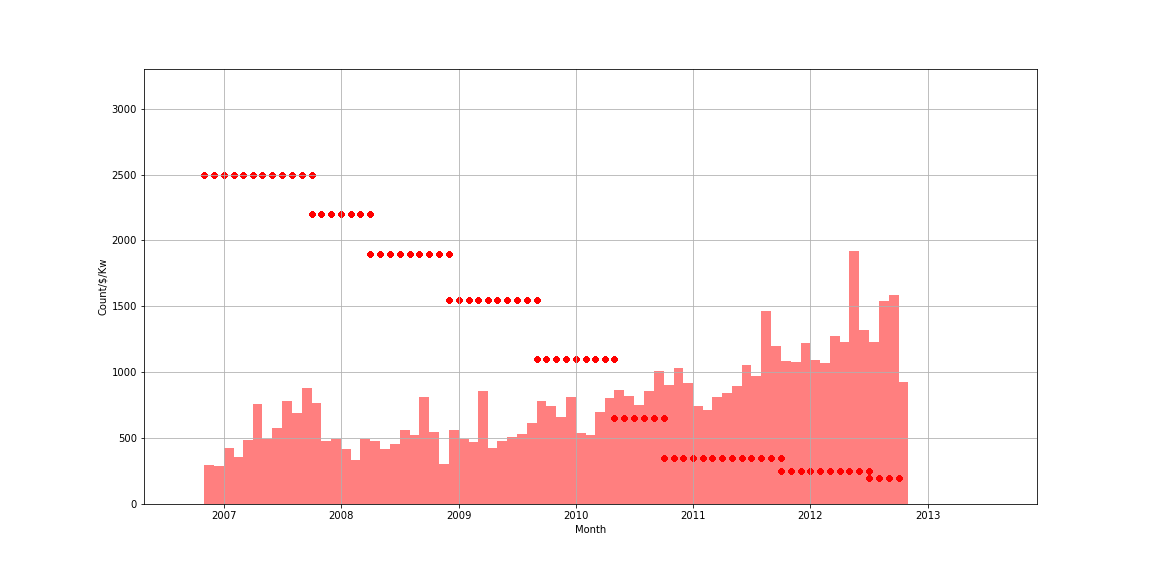
\includegraphics[width = 5in]{app_hist_pge}}\\
\subfloat[SDGE]{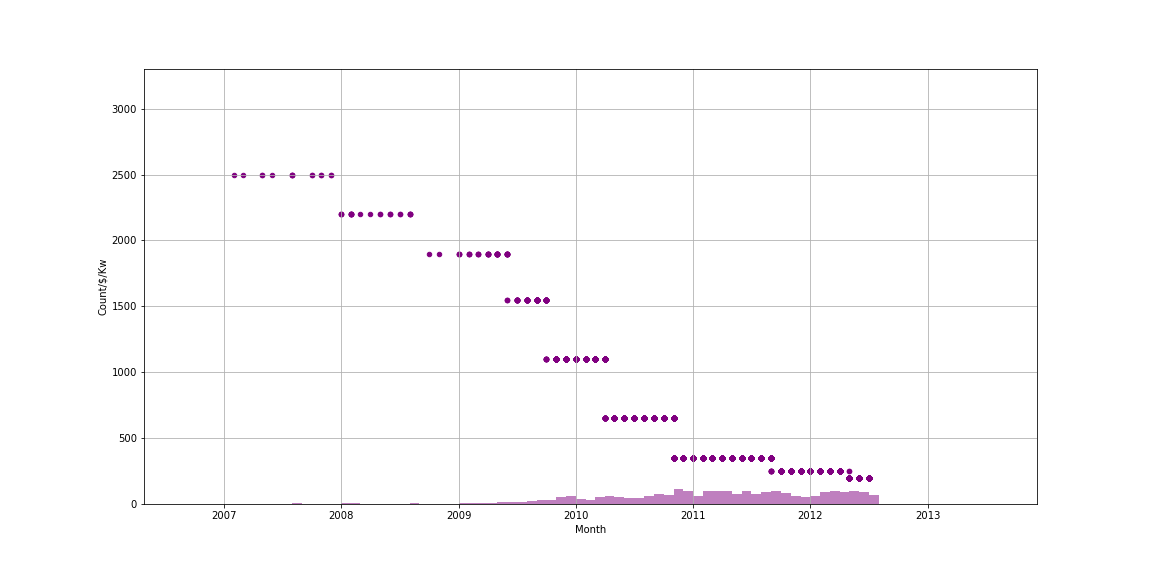
\includegraphics[width = 5in]{app_hist_sdge}}\\
\subfloat[ SCE]{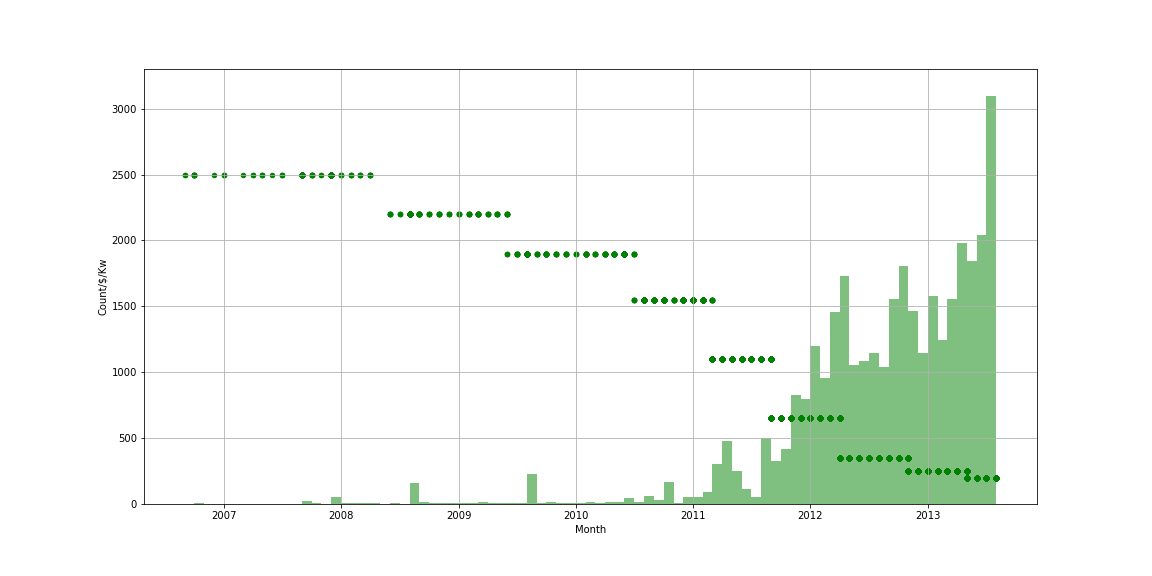
\includegraphics[width = 5in]{app_hist_sce}}\\
\end{tabular}

\end{center}
\caption{The bars are counts of applications received within a month. The dots are subsidy levels during month when applications were received.}
\label{cutoffs_and_apps}
\end{figure}

\subsection{Comparative Static}

I want to look at how the productivity of installers modulates the effect of a demand side subsidy. To do so, I take a comparative static of the first order condition of the model above with respect to an ad-valorum demand-side subsidy. The initial equation is

\[
\frac{D^{-1}(f(k,k)}{1-t} f_2(k,k) = r + \frac{w}{h'(C(k,k))} f_2 (k,k)
\]

Where $\frac{D^{-1}(f(k,k)}{1-t}$ is the price faced by the representative firm due to the inverse demand function that in equilibrium will influence the price level and the subsidy. To make the comparative static easier to calculate I'll assume the following functional forms.

\begin{align*}
&f(K,k) = K^\alpha k^\beta & \alpha+\beta >1, ~ 0<\beta<1 \\
&h(C) = C^\gamma & 0 < \gamma < 1 \\
&D^{-1} (y) = y^{-1}
\end{align*}

The assumption $\alpha+\beta >1$ is necessary to induce the increasing returns to R\&D within Romer's production function. With these functional forms, the first order condition becomes: 

\[
\frac{\beta}{(1-t)k} = r + w \frac{\beta}{\gamma} k^{\frac{\alpha+\beta}{\gamma} - 1}
\]

And the effect of a change in the level of the subsidy on the level of $k$ is:

\begin{equation}
\frac{dk}{dt} = \left[ \frac{1-t}{k} + (1-t)^2 \frac{w (\alpha + \beta - \gamma)}{\gamma^2} k^{\frac{\alpha+\beta}{\gamma} - 1} \right]^{-1} = +ve
\label{comp_stat}
\end{equation}

So as expected, when the subsidy increases the equilibrium amount of R\&D increases. And because there is a positive monotonic relationship between output and R\&D, output must increase as well. $\gamma$ is the productivity of installation activity, and from inspection you can see that when $\gamma$ increases, so does the magnitude of the comparative static.

The intuition behind this is as follows. As installer productivity increases, the marginal cost of the representative firm decreases, and so its supply curve shifts down and becomes more elastic. Thus, for any change in equilibrium price caused by the subsidy, the affect on R\&D and so output will be greater.

\subsection{Calculating Installer Productivity}

The model I have describes production at the industry level. For this reason, I aggregate installation data to the IOU-month level. I have data on the date each project in an IOU was applied for, and the date it was completed (Roberson 2015). If a project is completed within an IOU-month, I treat that as an amount of output. I look at two ways of classifying output: (1) the total size of the system installed in kilowatts, and (2) the total quantity of generators and inverters installed. These two outcomes are highly correlated, but given the technological progress influencing the efficiency of equipment, it seemed prudent to look at both. This analogue to this output in my theory above is $h(C)$. I define the analogue to $C$ as the amount of output concurrently committed to in an IOU-month. By that mean, the number of projects that are either completed in a month, or have their application reception date during/before the IOU-month and the completion date after. So, if SCE completed 60 Kw of installations in July, and during that month they had applications totaling an additional 40 Kw that they were committed to installing, but have not gotten to yet, then $C= 100$ $h(C) = 40$.  In defining `hired capacity' $C$ in this way, I am assuming that the costs to installers of each unit of size installed or equipment installed are linear. In defining output $h(C)$ in this way, I am restricting output to be weakly less than hired capacity. I then calculate the best linear fit of output to capacity hired.

\[
y_{im} = \alpha + \gamma c_{im}
\]

$y_{im}$ is the sum in IOU $i$ during month $m$ of completed system size or quantity of equipment. $c_{im}$ is the sum of system size or quantity of equipment committed to during month $m$ in IOU $i$. I restrict data to applications declaring they are not self installing, indicating that they have hired a firm to install their systems. In this way, $\gamma$ is then the linear best fit of productivity of hired capacity.

Figure \ref{agg_prod_fig} visualizes the results of estimating the above econometric model. Table \ref{agg_prod_tab} displays the estimates themselves. This is a rough analysis, but it indicates that the installation industry in SCE is more productive than in PGE, and that SDGE is far more productive than both. The very high estimated productivity of SDGE calls into question that I have a representative sample in SDGE. I need to look further into the data in SDGE.

\begin{figure}
\begin{center}
Aggregate Installer Productivity Per Month By IOU
\begin{tabular}{cc}
\subfloat[Quantity of equipment installed in PGE]{\includegraphics[width = 3in]{q_comp_PGE}} &
\subfloat[Total size installed in PGE]{\includegraphics[width = 3in]{size_comp_PGE}}\\
\subfloat[Quantity of equipment installed in SCE]{\includegraphics[width = 3in]{q_comp_SCE}} &
\subfloat[Total size installed in SCE]{\includegraphics[width = 3in]{size_comp_SCE}}\\
\subfloat[Quantity of equipment installed in SDGE]{\includegraphics[width = 3in]{q_comp_SDGE}} &
\subfloat[Total size installed in SDGE ]{\includegraphics[width = 3in]{size_comp_SDGE}}\\
\end{tabular}
\end{center}
\caption{The y-axis is the sum of the total system size or equipment installed by installers in a month in an IOU. The x-axis is the sum of the total system size or equipment that installers were committed to installing during that month, according to subsidy applications. For example, If an installers in an IOU installed 40 Kw of system in July 2010, and were named on subsidy applications for projects totaling another 60 Kw in system size in that IOU during July 2010, then the observation for that IOU-month-year has 40 Kw installed, and 100 Kw committed to. Note this means that installed projects are counted as commitments. Axes are scaled symmetrically and identically so as to fit all data and allow comparison. The blue points are IOU-month-year observations. The red line is the best linear fit.}
\label{agg_prod_fig}
\end{figure}

\begin{table}
\begin{center}
Aggregate Installer Productivity Per Month By IOU

\vspace{0.5cm}

A. Total Size (DC, Kw) of Systems Installed Per Month, 

Per Total Size Committed to Per Month, By IOU

\vspace{0.25cm}

\subimport{term_paper_analysis/}{size_comp_res}

\vspace{0.5cm}

B. Quantity of Equipment Installed Per Month, 

Per Quantity Committed to Per Month, by IOU

\vspace{0.25cm}

\subimport{term_paper_analysis/}{q_comp_res}
\end{center}
\caption{}
\label{agg_prod_tab}
\end{table}

But, the implication that I move forward with is that the installation industry in SDGE is by far the most productive, SCE is the second most, and PGE is the least.

\subsection{The Conditional Correlation Between Subsidy Level and Output}

Looking at the histograms shown in figure \ref{cutoffs_and_apps}, there is evidence of a time trend, seasonality, and yearly idiosyncrasies in the number of applications. For these reasons, I estimate the following equation, separately for each IOU. Observations are now at the application level

\begin{equation}
log(y_i) = \alpha + \beta ~ log(subsidy_i) + \vec{\omega} + \vec{\eta} + \delta~ t + \epsilon
\end{equation}

$y_i$ is either the total system size or total quantity of generators and inverters installed for a single application. $subsidy_i$ is the level of the CSI subsidy at the time the application was received, in dollars per watt. The conditional correlation of these outcomes with the subsidy level will be captured by the coefficient $\beta$. $\vec{\omega}$ and $\vec{\eta}$ are vectors of month and year fixed effects, respectively, and $\delta$ is the coefficient on the time trend. I treat a month as the unit of time. $\epsilon$ is the error term.

\begin{table}
\begin{center}
Effect of Subsidy on Solar Industry Output

\vspace{0.5cm}

A. Effect on Total Size (DC, Kw) of Subsidy (\$/Watt), by IOU

\vspace{0.25cm}

\begin{tabular}{llll}
\hline
               & PGE      & SDGE     & SCE       \\
\hline
log\_subsidy   & 0.0922   & 0.2246   & -0.3465   \\
               & (0.0247) & (0.1315) & (0.0213)  \\
R-squared      & 0.0087   & 0.0330   & 0.0838    \\
R-squared Adj. & 0.0082   & 0.0259   & 0.0832    \\
N              & 56037    & 2604     & 34270   
\\ \hline
Month Fixed Effects & Yes & Yes & Yes \\ 
Year Fixed Effects & Yes & Yes & Yes \\
Month Time Trend & Yes & Yes & Yes \\ \hline
Installer Productivity (Size) & 0.1766 & 0.9643 & 0.1850 \\ \hline
\end{tabular}

\vspace{0.5cm}

B. Effect on Quantity Installed of Subsidy (\$/Watt),, by IOU

\vspace{0.25cm}

\begin{tabular}{llll}
\hline
               & PGE      & SDGE     & SCE       \\
\hline
log\_subsidy   & -0.0657  & 0.2826   & 0.0274    \\
               & (0.0272) & (0.1344) & (0.0115)  \\
R-squared      & 0.0122   & 0.0214   & 0.0127    \\
R-squared Adj. & 0.0119   & 0.0146   & 0.0121    \\
N              & 56037    & 2604     & 34270   
\\ \hline
Month Fixed Effects & Yes & Yes & Yes \\ 
Year Fixed Effects & Yes & Yes & Yes \\
Month Time Trend & Yes & Yes & Yes \\ \hline
Installer Productivity (Quantity) & 0.2131 & 0.9621 & 0.2452 \\ \hline
\end{tabular}

\end{center}
\caption{Regression takes place using individual CSI subsidy applications as observations. Outcome of interest is either the logarithm of total size of system installed, or the logarithm of total quantity of generators and inverters installed. The independent variable of interest is the logarithm of the subsidy. Subsidy is $\$/Watt$. The estimated productivity of installers is included in the last line of each table. IOUs with higher productivity have a higher correlation between demand and subsidy level.}
\label{subsidy_table}
\caption{}
\end{table}


The month and year fixed effects and the time trend reference the date the application was received completed. The price, system size, and quantity of equipment are agreed upon at this date, and so this is when the subsidy would have its effect. 

The results of the estimation are shown in table \ref{subsidy_table}. I do estimate a negative coefficient of interest in half of the results. This indicates I have not properly controlled for the spurious correlation caused by the decrease in subsidies and increase in demand over time. But, the IOUs that were estimated to have a higher productivity in the previous section have a more positive correlation between subsidy level and output than those estimated to have lower productivity. This is promising, and indicates that the productivity of installers may increase the effect of a demand-side subsidy on demand.


\section{Conclusion}

This is only a preliminary analysis of the theory and empirics of the solar supply chain and empirics of the supply chain. It shows that there is potential for research that can inform optimal subsidization on the solar supply chain. In future research, I hope to improve the theory and empirics. 

Empirically, the data also have information on the equipment installed, including the model and manufacturer. Many solar manufacturers are publicly traded in the US, and so have to file a 10-K form with the SEC. in these filings, companies often report their spending on R\&D. It may be possible to use this data to study the contributions of both installation capacity and manufacturer R\&D, and so to make an empirically backed claim on how to optimize the solar supply chain in order to increase output.


\begin{thebibliography}{1}

\bibitem{} Branstetter, Lee G. "Are knowledge spillovers international or intranational in scope?: Microeconometric evidence from the US and Japan." Journal of International Economics 53.1 (2001): 53-79.

\bibitem{} Keller, Wolfgang. "Knowledge spillovers at the world's technology frontier." Available at SSRN 271703 (2001).

\bibitem{} Los, Bart, and Bart Verspagen. "R\&D spillovers and productivity: evidence from US manufacturing microdata." Empirical economics 25.1 (2000): 127-148.

\bibitem{} Romer, Paul M. "Increasing returns and long-run growth." Journal of political economy 94.5 (1986): 1002-1037.

\bibitem{} Roberson, Tim 2015. Currently being rewritten and so unavailable.

\end{thebibliography}

\end{document}